%
% durchstosspunkt.tex
%
% (c) 2018 Prof Dr Andreas Müller, Hochschule Rapperswil
%
\documentclass[tikz]{standalone}
\usepackage{times}
\usepackage{amsmath}
\usepackage{txfonts}
\usepackage[utf8]{inputenc}
\usepackage{graphics}
\usetikzlibrary{arrows,intersections,math}
\usepackage{ifthen}
\begin{document}

\newboolean{showgrid}
\setboolean{showgrid}{false}

\begin{tikzpicture}[>=latex,thick]

% Povray Bild
\node at (0,0) {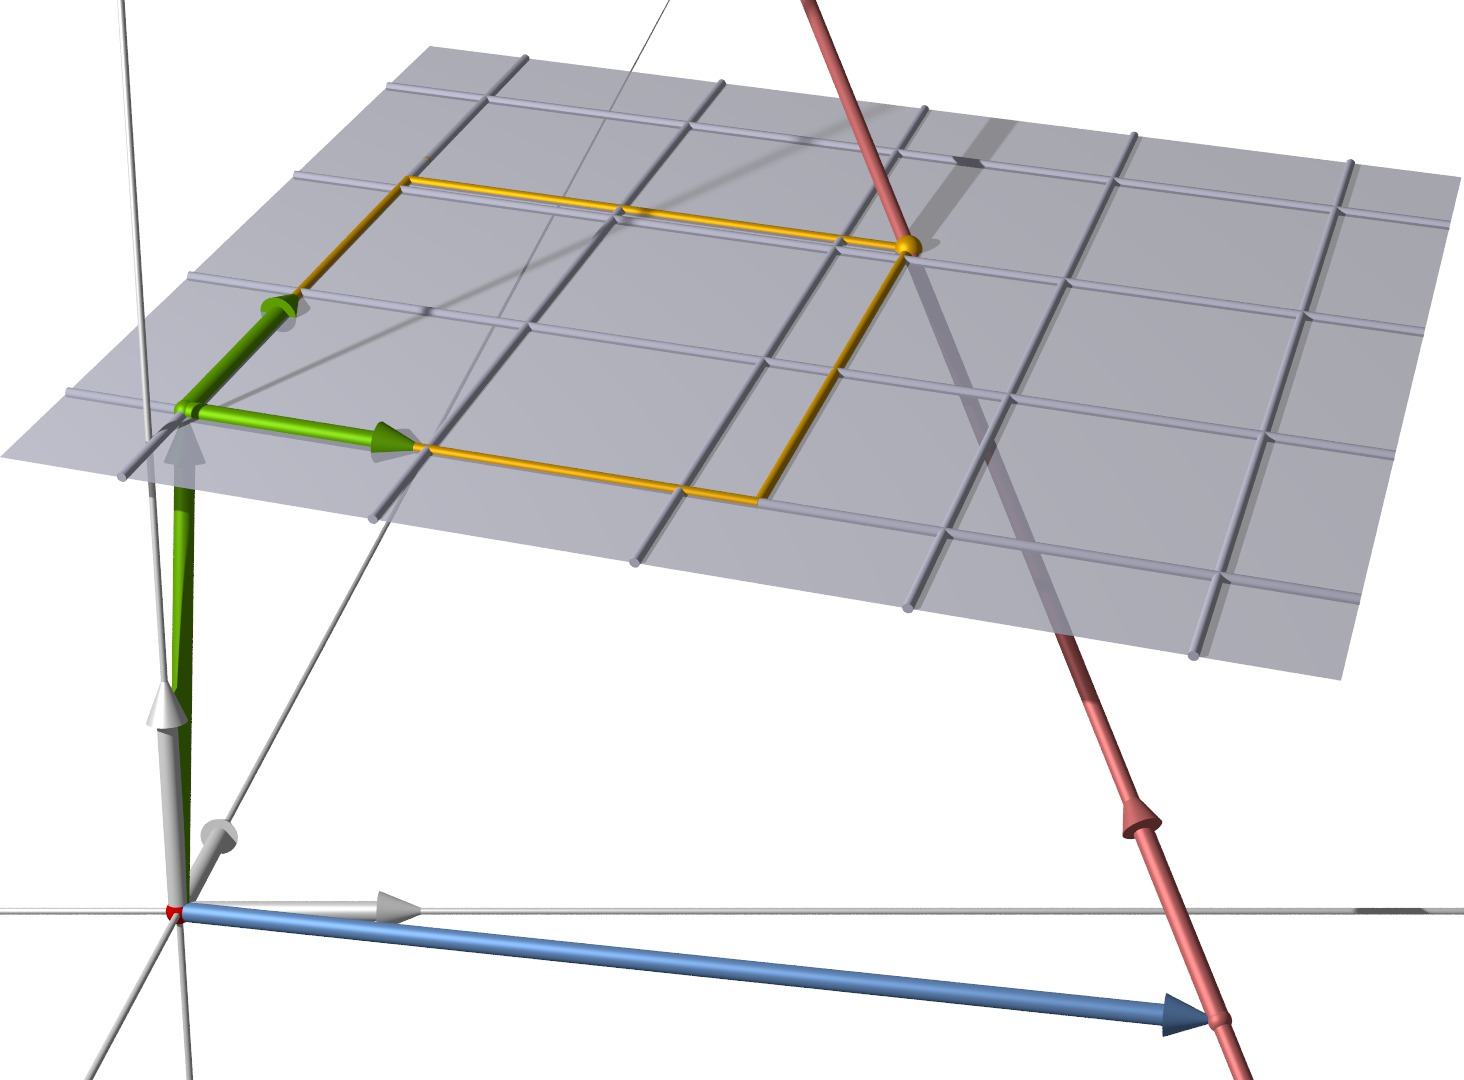
\includegraphics[width=14cm]{durchstosspunkt.jpg}};

% Gitter
\ifthenelse{\boolean{showgrid}}{
\draw[step=0.1,line width=0.1pt] (-7,-5) grid (7, 5);
\draw[step=0.5,line width=0.4pt] (-7,-5) grid (7, 5);
\draw (-7,-5) grid (7, 5);
\fill (0,0) circle[radius=0.05];
}{}

% Ebene
\node at (-4.7,2.5) {$\vec{u}$};
\node at (-3.1,1.2) {$\vec{v}$};
\node at (-5.3,1.6) {$P_0$};
\node at (-4.9,-0.3) {$\vec{p}_0$};
\node at (6.4,3.3) {$\sigma$};

% Gerade
\node at (4.9,-4.2) {$Q_0$};
\node at (4,-2.2) {$\vec{r}$};
\node at (3.5,-4.9) {$\vec{q}_0$};
\node at (1.2,4.8) {$g$};

% Durchstosspunkt
\node at (2, 3) {$S$};
\node at (0.1,0.1) {$s\vec{v}$};
\node at (-3.4,3.5) {$t\vec{u}$};

\end{tikzpicture}

\end{document}

